% !TeX root = ../../main.tex
% Add the above to each chapter to make compiling the PDF easier in some editors.

\section{Semantic Segmentation}\label{ord:ch2:sec2}

\subsection{Motivation}\label{ord:ch2:sec2:subsec_motivation}
Semantic segmentation finds application in various tasks and is widely used over different domains.
Due to its capability to perform classification on pixel-level it is often applied on scene understanding \cite{LiJ09-SceneUnderstanding} or the evaluation of satellite images \cite{Li18-SateliteImagery}.
In the field of autonomous driving semantic segmentation is used for street scene analysis \cite{Cor16-Cityscapes} \cite{Men15-AutonVehicles} \cite{Neu17-MapillaryDataset}.
In medicine this method can be used to segment cancer cells, tumors \cite{RF15-U-Net} or blood cells \cite{Tran19-BloodCell}.
Further, it is applied in order to fulfill abstract tasks like the reconstruction of indoor scenes \cite{Dai17-ReconstructionIndoorScenes}.
This listing of only some applications gives an idea of how versatile and functional image segmentation is and what can be achieved with it in the future.


\subsection{General}\label{ord:ch2:sec2:subsec_general}
Image segmentation is an advanced task of computer vision.
The goal of segmentation algorithms is to obtain regions of interest from an image.
In order to partition the image into regions, a high level of understanding is required.
Modern techniques of \gls{dl} have proven themselves to be most adequate for this task.
Today, for image segmentation deep \glspl{cnn} are applied.
There two main variants to perform segmentation on images:
\begin{itemize}
	% Semantic segmentation
	\item \textbf{Semantic segmentation} classifies each pixel with one class \cite{RF15-U-Net} \cite{Zhao17-PSP}, illustrated in Figure \ref{fig:ch2:sec2:semantic_seg}.
	There is no differentiation made if there are multiple objects of one class, they all belong to the same region.
	% Instance segmentation
	\item \textbf{Instance segmentation} differentiates between different objects object instances \cite{DHS16-MNC} \cite{He17-MaskR-CNN} as shown in Figure \ref{fig:ch2:sec3:instance_seg}.
	Each instance has its own region and a label of the corresponding class $k$.
	In the result several regions may have the same class, but are treated as independent instances of this class.
\end{itemize}

This thesis deals with the labeling of objects and therefore, it is further not distinguished between semantic and instance segmentation.
This is why, the labeling process of an instance may also be seen as semantic segmentation on a limited domain.
\begin{figure} [h]
	\centering
	\begin{subfigure}[t]{0.3\textwidth}
		\centering
		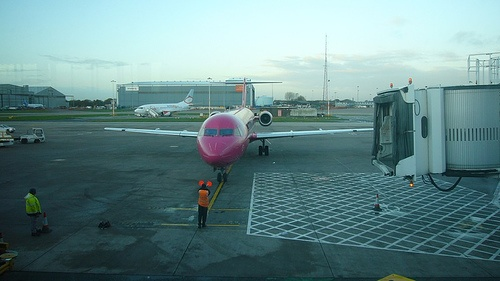
\includegraphics[width=\textwidth]{figures/chap22_image.jpg}
		\caption{
			Input image $\textbf{x}$
		}\label{fig:ch2:sec2:image}
	\end{subfigure}
	\hfill
	\begin{subfigure}[t]{0.3\textwidth}
		\centering
		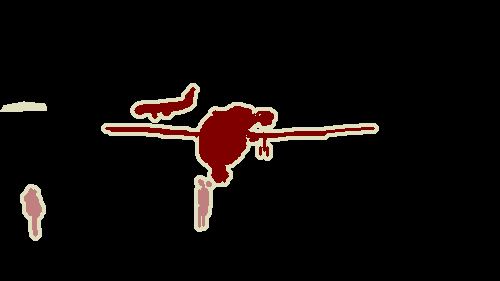
\includegraphics[width=\textwidth]{figures/chap22_semantic_seg.png}
		\caption{
			\gls{gt} for semantic segmentation.
			Each class has a label of the same color.
		} \label{fig:ch2:sec2:semantic_seg}
	\end{subfigure}
	\hfill
	\begin{subfigure}[t]{0.3\textwidth}
		\centering
		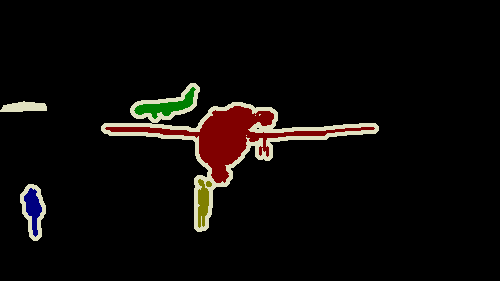
\includegraphics[width=\textwidth]{figures/chap22_instance_seg.png}
		\caption{
			\gls{gt} for instance segmentation.
			Each instance has a different colored label.
		}\label{fig:ch2:sec3:instance_seg}
	\end{subfigure}
	\caption[Semantic and instance segmentation]{
		Sample images of the PASCAL \glsentryshort{voc} Dataset \cite{Eve20-PascalVOC}, that distinguish between semantic and instance segmentation.
		The background class is colored back.
		The white class are the \glsentryshort{vp}, that are around boundary of the object.
	}\label{fig:ch2:sec2:segmentation_image}
\end{figure}

% Supervised-learning, data with labels on pixel-level.
For this thesis methods that are trained in a supervised manner are of interest.
Therefore, a dataset with labels for each image on pixel-level is required.
A label $y$ is represented by a map, which is an image of the same size as the input image $\textbf{x}$ and where each pixel has class label $y_{rc}$ with $r$ and $c$ referring to the corresponding row and column of the map. 
In this context the label $y$ is also referred to as mask or \gls{gt}.
Segmentation is treated as a classification task with $K$ classes.
The model creates a prediction $\hat{y}$, that also represented by a map, similar to the map $y$.
In this map a class $k$ is predicted for each pixel $\hat{y}_{rc}$.
Pixels with a the same class label form a region, that may be further processed afterwards.

% Loss function.
To train a segmentation network a loss function is required, that considers the loss of every pixel in the image and optimizes the prediction for each pixel individually.
In \cite{Jad20-LossFunction} several loss functions for image segmentation are examined.
Jadon concludes, that there is no universal loss function, instead their performance depends on the characteristics of the dataset.
Cross entropy loss works best on a balanced dataset, while for imbalanced datasets the dice coefficient or focal loss is suitable.

% TODO introductional sentence that this is important for the architecture???
The task of semantic segmentation aims to answer the questions of classification \emph{what is in the image?} and the question of localization \emph{where is it in the image?}.
The network extracts features and learns to answer the question of classification.
During this process the size of feature maps decrease and localization information is lost.
As a result it gets harder to perform a detailed reconstruction and answers the question of localization.
Architectural solutions to solve to solve this problem are introduced in Section \ref{ord:ch2:sec2:subsec_arch}.

\paragraph{PASCAL VOC Dataset}

% Basic description
The PASCAL \glsentryfull{voc} Challenge \cite{Eve20-PascalVOC} is established as a frequently used benchmark for the tasks of image classification, detection, and segmentation.
Due to this variety in application, the PASCAL \gls{voc} Challenge enjoys great popularity in the \gls{dl} community.
From 2005 to 2012 an annual challenge was created with an annual advanced dataset.
Despite the last release is almost a decade ago, the PASCAL \gls{voc} 2012 dataset is still to evaluate state-of-the-art methods and is used a benchmark for comparisons.
Due to the large use in recent years, this dataset also plays an important role in this thesis.
A sample with image and labels from the PASCAL \gls{voc} 2012 dataset is shown in Figure \ref{fig:ch2:sec2:segmentation_image}
% Size (iamges and annots) and label types
For the task of segmentation this dataset contains 6,929 annotations from 20 classes.

% Some times questionable labels of bicycles and plants
Despite the PASCAL \gls{voc} 2012 dataset is fairly popular, it features certain disadvantages, which must be taken into account for a fair evaluation.
First, the quality of some single annotations is questionable.
It was experienced, that especially for thin, long objects (\eg plants or the spite of bicycle wheels) the \gls{gt} partly seems inaccurate.
% often used for evaluation -> careful because general use datatset
Second, the PASCAL \gls{voc} datasets have so-called \gls{vp}, that are located around each object as a boundary, as illustrated in Figure \ref{fig:ch2:sec2:segmentation_image}.
They were established to prevent the inclusion of wrongly labeled \gls{gt} pixels, as label inaccuracies especially take place around the boundary of the object.  
\gls{vp} are excluded from the training and evaluation, which leads to a distorted evaluation result.
In most comparisons the presented results on PASCAL \gls{voc} datasets are created with the application of \gls{vp}.
This does not lead to a realistic evaluation, since the boundary, which is particularly difficult to segment, is ignored.
Evaluating the performance, this must be taken into account, because real world data do have \gls{vp}. 
In Section \ref{ord:ch5:sec2_generalization_image_domains}, experiments demonstrate, that the performance significantly drops without the use of \gls{vp}.
% TODO ref appendix for examples

\subsection{Evaluation Metric}\label{ord:ch2:sec2:subsec_metric}
To ensure an objective comparison of several methods a evaluation metric is required, which measures the quality of obtained segmentation.
% OP
As this challenge is a classification task on pixel-level, a measure of evaluation is the \gls{op} accuracy, which represents the proportion of all correctly labeled pixels in an image or a whole dataset.
% "One significant limitation of this measure is its bias in the presence of very imbalanced classes. This is the case for the background class on PASCAL VOC datasets, which covers 70-75% of all pixels" \cite{Csu13-EvalMetric}
% PC
Further, the \gls{op} measurement can be refined by calculating the accuracy for each class.
This results in the \gls{pc} accuracy, which represents the proportion of correctly labeled pixels of one class.
% AP
% Another metric is the \gls{ap} 
%Another common metric is the \textit{Precision}, which the accuracy of the positive predictions and defined as
%\begin{equation}
%	Precision = \frac{\textnormal{true positives}}{\textnormal{true positives} + \textnormal{ false positves}}
%\end{equation}

% IoU
The most commonly used evaluation metric is the \gls{iou}, also known as the Jaccard Index, which is used in the PASCAL VOC challenge \cite{Eve20-PascalVOC} since 2008 \cite{Csu13-EvalMetric}. 
The \gls{iou} measures the ratio of overlap (true positives) between \gls{gt} and prediction $\hat{y}$ and of the total area. 
It is defined as
\begin{equation} \label{equ:iou}
	\centering
	IoU = \frac{\textnormal{\textit{true positives}}}{\textnormal{\textit{true positives}} + \textnormal{\textit{false negatives}} + \textnormal{\textit{false positves}}}
\end{equation}
and is calculated for each instance or segmentation class.
To evaluate all instances or classes of an image or a dataset the \gls{iou} is averaged, which results in the \gls{miou}.\footnote{An open source implementation can be found, \eg in TensorFlow: \textit{tf.keras.metrics.MeanIoU}: \url{https://www.tensorflow.org/api_docs/python/tf/keras/metrics/MeanIoU}}
%TODO other reference here than open source stuff??

\begin{figure}
	\centering
	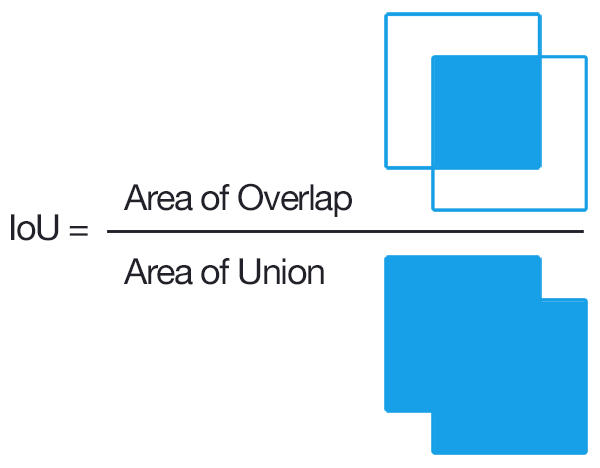
\includegraphics[width=0.5\textwidth]{figures/chap222_iou.png}
	\caption[Intersection over Union]{
		\glsentrylong{iou}. The \textit{area of overlap} represents the intersection of the \gls{gt} with the made prediction $\hat{y}$. 
		The \textit{area of union} represents the total area of \gls{gt} and the prediction $\hat{y}$ \cite{Sha18-DLCV}. \textit{TODO recreate a visualization like this by myself}}
	\label{fig:ch2:sec2:iou}
\end{figure}
% TODO get licence or change grafic 

An advantage of this metric is the inclusion of \textit{false positives} and \textit{false negatives} into the calculation.
A limitation of the \gls{iou} metric is that the boundary correctness of the region's boundaries is not taken into account. 
In order to compensate this issue, Csurka suggests in \cite{Csu13-EvalMetric} to combine the \gls{iou} with another complementary metric, evaluating the boundary of a region.
Regardless, the \gls{iou} is a suitable and informative metric, which is also the most common to evaluate semantic segmentation models.



\subsection{Semantic Segmentation Architectures}\label{ord:ch2:sec2:subsec_arch}
\gls{cnn} architectures for image classification follow a common scheme: 
A multi dimensional input image $\textbf{x}$ is processed and continuously downsized to a one dimensional tensor, in order to make one prediction $\hat{y}$.
In contrast, for image segmentation a prediction is made for each pixel of the image.
Therefore, an adaption of the architecture required, that enables the model to make a prediction for every pixel of the image $\hat{y}_{rc}$.
In the following characteristics of important architectures and components are examined.

\subsubsection{Encoder-Decoder-Architecture}
The Encoder-Decoder-Architecture as its name anticipates is based on two main parts: the encoder network and the decoder network, exemplary visualized in Figure \ref{fig:ch2:sec2:encoder-decoder}. 
Representatives of the encoder-decoder-architecture are U-Net \cite{RF15-U-Net}, DeConvNet \cite{NHH15-DeConvNet} and SegNet \cite{Bad17-SegNet}.

The encoder network is the feature extraction part of a classification \gls{cnn}.
It consists out of convolution and pooling layers, that reduce the size of the feature maps and extract features.
Therefore, the encoder network is the classification backbone and for DeConvNet \cite{NHH15-DeConvNet} and SegNet \cite{Bad17-SegNet} the backbone is based on VGG-16 \cite{SZ15-VGG16}. 
In this context the process of applying the encoder network is also called \textit{downsampling}, due to the size reduction of the feature maps.

The decoder network is the counterpart of the encoder network.
It reconstructs the feature maps to their original size, which is also referred to as \textit{upsampling}.
To reach the input size often a reversed architecture of the encoder network is used.
The basic components of this reconstruction are the operations \textit{unpooling} and \textit{transposed convolution}, introduced in the following.

After the encoder network generally a softmax classifier is applied, that predicts the class for each pixel.
The output is a probability map $\hat{y}$ with $K$ channels for $K$ number of classes \cite{Bad17-SegNet}.

\begin{figure}
	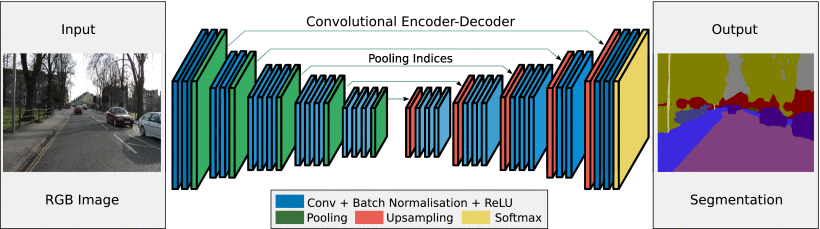
\includegraphics[width=\linewidth]{figures/chap223_segnet_arch.png}
	\caption[Encoder-Decoder-Architecture]{
		Encoder-Decoder-Architecture from SegNet. 
		On the left the encoder network, which reduces the size of the feature maps while processing. 
		On the right is the decoder network, which reconstructs the feature map to the size of the original input. 
		The yellow layer on the very right is the classification layer, here represented as softmax layer to create the output segmentation. 
		Copyright \copyright 2017 Creative Commons License. Reprinted by permission from \cite{Bad17-SegNet}.}
	\label{fig:ch2:sec2:encoder-decoder}
\end{figure}

\paragraph{Unpooling.}
The unpooling operation is the equivalent of the pooling operation.
Instead of reducing the size of feature maps $F^{n}_{c}$, they are enlarged.
As for pooling, no features are learned and there exist multiple methods to perform unpooling, two of them are illustrated in Figure \ref{fig:ch2:sec2:unpooling_1}.
Nevertheless, unpooling is not capable to fully reconstruct the information lost during the process of downsampling.
The result for \textit{bed of nails} are sparse feature maps $F^{n}_{c}$, while for \textit{nearest neighbor} the feature maps $F^{n}_{c}$ contain redundant information.
% In order to achieve a fine and detailed segmentation result, this is an interfering effect.
%For an architecture with max pooling and a mirrored structure of encoder and decoder network, this effect can be mitigated by saving the location of the maximal value during max pooling.
% In the following the unpooling result can be specified based on this information, as exemplified in Figure \ref{fig:ch2:sec2:unpooling_2} \cite{NHH15-DeConvNet} \cite{Fer19-SemSeg}.

% TODO recreate figure by myself with drawing program.
\begin{figure}
	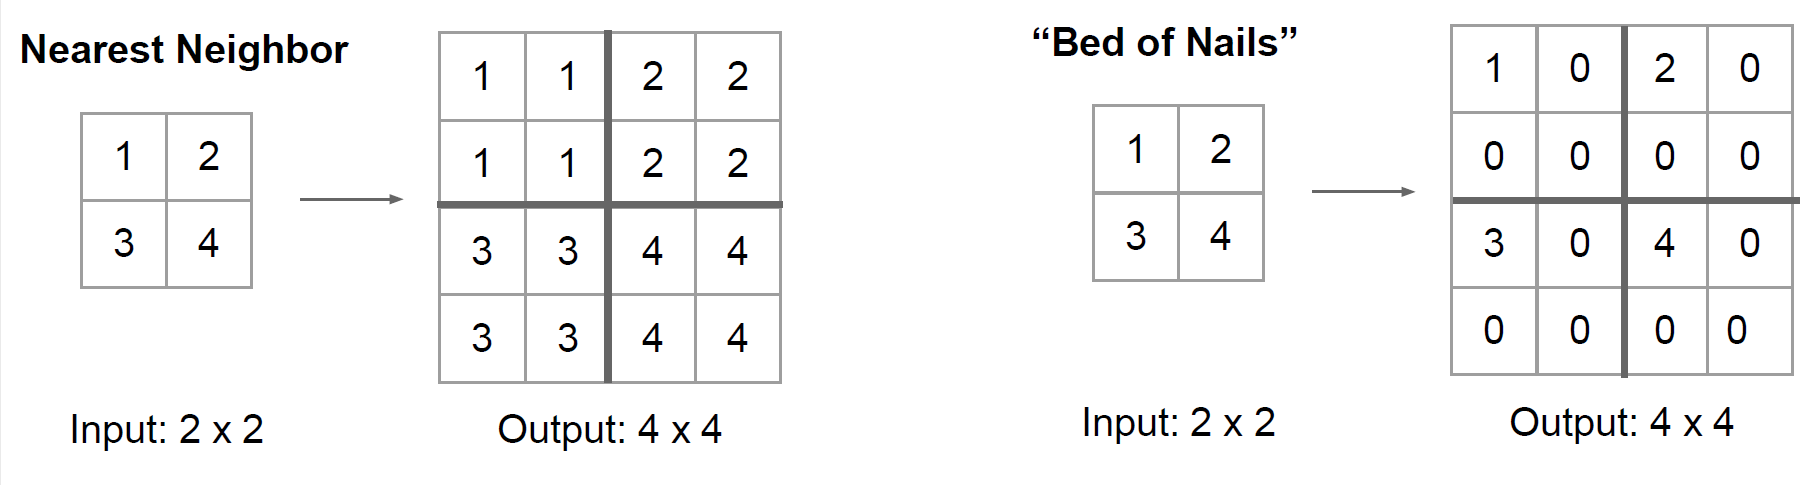
\includegraphics[width=\linewidth]{figures/chap223_unpooling1.png}
	\caption[Unpooling methods \textit{nearest neighbor} and \textit{bed of nails}]{
		Unpooling methods \textit{nearest neighbor} and \textit{bed of nails}.
		With \textit{nearest neighbor} enlarged feature maps are filled up with the same input value. 
		With \textit{bed of nails} sparse feature maps are created, that contain the input value filled up with zeros.
		\textit{TODO recreate figure with drawing program}}	
	\label{fig:ch2:sec2:unpooling_1}
\end{figure}
% \footref{fn:LJY10_StanfordLecture}
%	\footnotemark{\ref{footnote:LJY10_StanfordLecture}} 

% \begin{figure}
% 	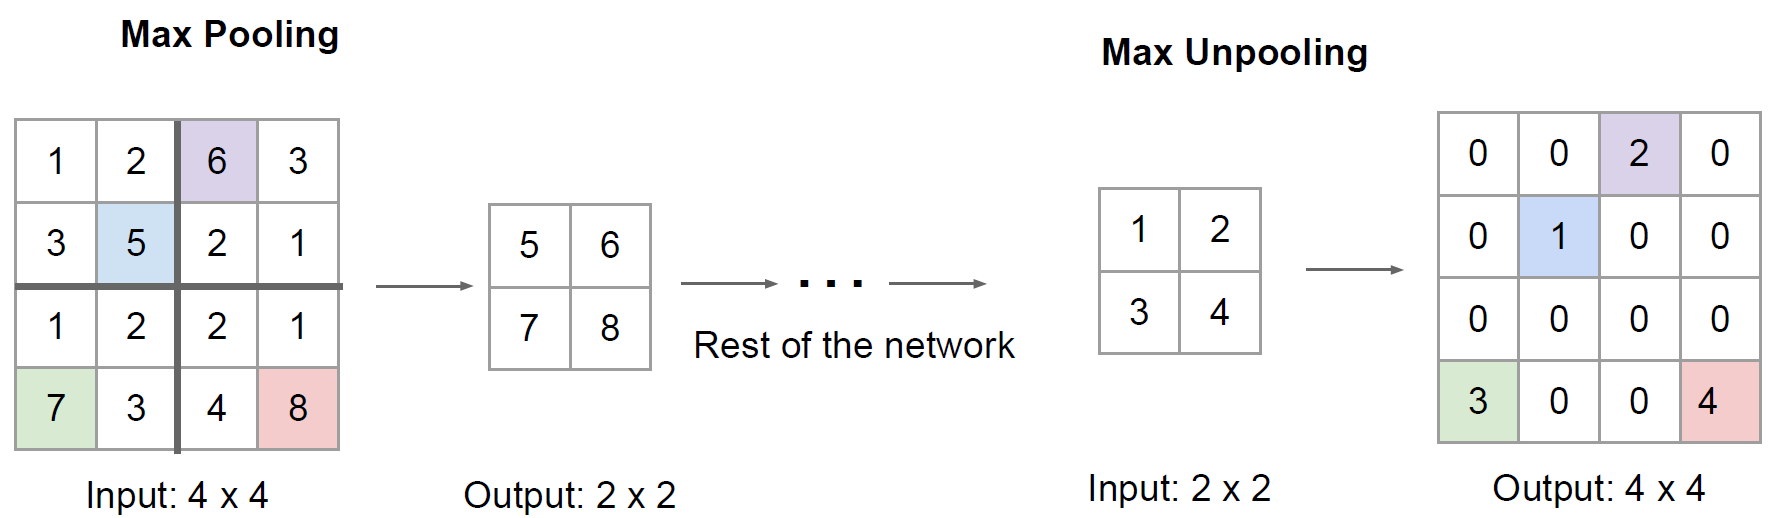
\includegraphics[width=\linewidth]{figures/chap223_unpooling2.png}
% 	\caption[Max Unpooling]{\textit{Max unpooling} \cite{Li17-StanfordLecture}. During max pooling the location of the maximal element is remembered. During max unpooling this location-information is reapplied to achieve a specified result, compared to the \textit{bed of nails} method.}
%	\label{fig:ch2:sec2:unpooling_2}
%\end{figure}

% We can observe that coarse-tofine object structures are reconstructed through the propagation in the deconvolutional layers; lower layers tend to capture overall coarse configuration of an object (e.g. location, shape and region), while more complex patterns are discovered in higher layers. 
% Note that unpooling and deconvolution play different roles for the construction of segmentation masks. Unpooling captures example-specific structures by tracing the original locations with strong activations back to image space. As a result, it effectively reconstructs the detailed structure of an object in finer resolutions. On the other hand, learned filters in deconvolutional layers tend to capture class-specific shapes. Through deconvolutions, the activations closely related to the target classes are amplified while noisy activations from other regions are suppressed effectively. By the combination of unpooling and deconvolution, our network generates accurate segmentation maps \cite{NHH15-DeConvNet}.

\paragraph{Transposed Convolution.}
As for pooling it is unpooling, the counterpart of convolution is transposed convolution.
Therefore, these operations also share common features and characteristics, like learnable filters or hyperparameters as \textit{kernel size}, \textit{padding} and \textit{stride}.
Transposed convolution can be used to enlarge feature maps or dense sparse feature maps, as created by the unpooling method "bed of nails".
% TODO clarify if Noh or Noh et al.
% Purpose of transposed conv for reconstruction.
In \cite{NHH15-DeConvNet} it is observed, that the lower layers of the decoder network handle coarse details (\eg location, shape and region), while the higher layers capture the fine and more complicated details.
This leads to a coarse-to-fine approach for the reconstruction through the decoder network.
In literature transposed convolution is also referred to as  \textit{deconvolution} \cite{NHH15-DeConvNet}, \textit{inverse convolution} \cite{Bad17-SegNet} or \textit{backwards convolution} \cite{LSD15-FCN}.
A visualization of transposed convolution is provided in \cite{DV19-ConvolutionGuide}.
% \footnote{F.-F. Li, J. Johnson and S. Yeung, 2018, "Stanford Lecture Detection and Segmentation": \url{http://cs231n.stanford.edu/slides/2018/cs231n_2018_lecture11.pdf}\label{fn:LJY10_StanfordLecture}}.

% TODO recreate figure by myself with drawing program.
\begin{figure}
	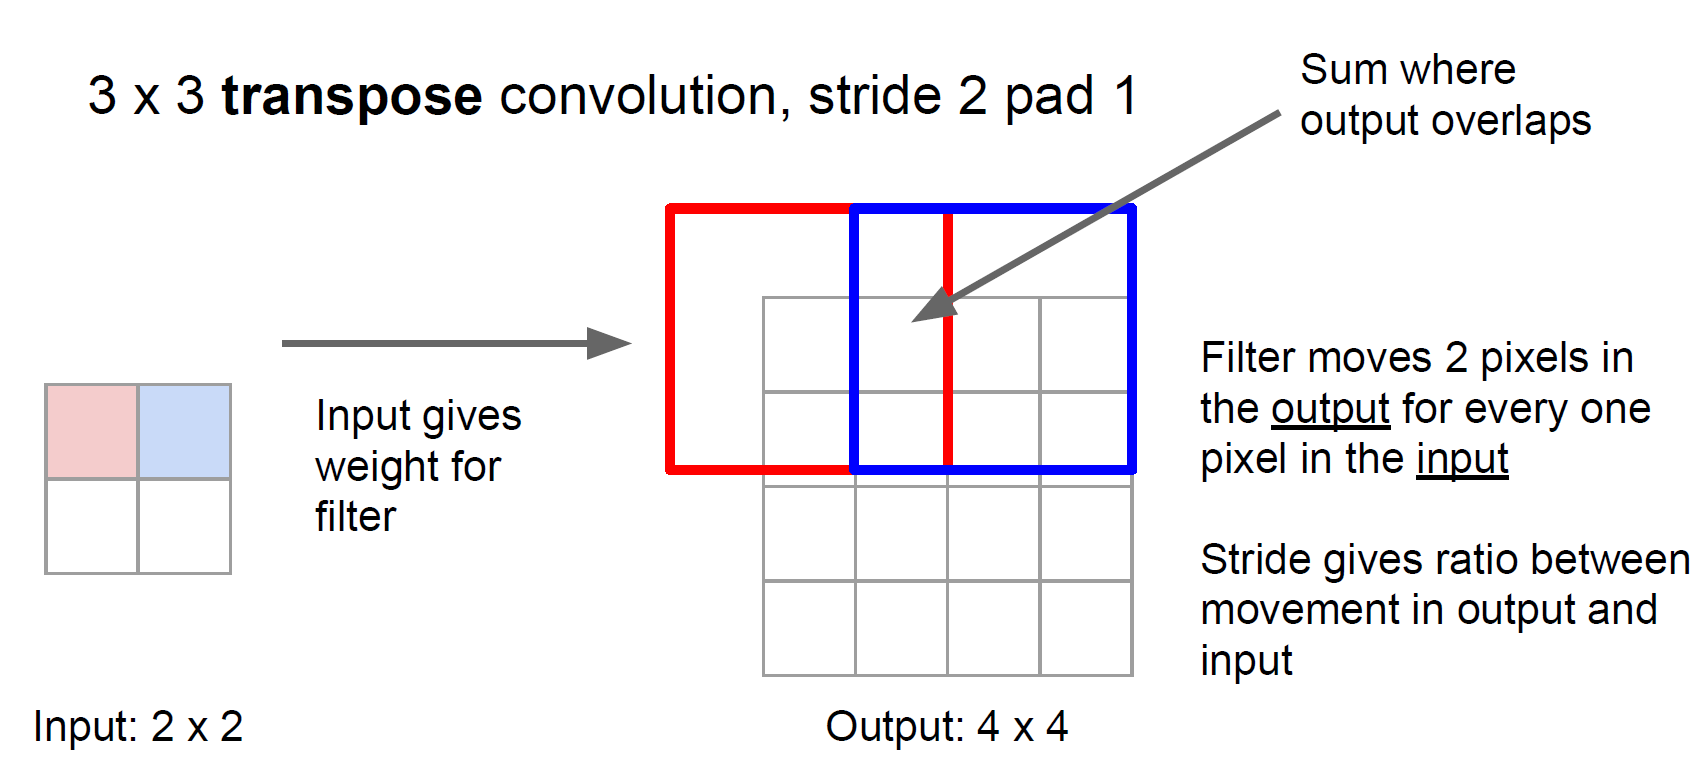
\includegraphics[width=\linewidth]{figures/chap223_transpose_conv.png}
	\caption[Transposed Convolution]{
		Example of the transposed convolution with $\textnormal{\textit{kernel size}} = 3 \times 3$, $stride = 2$ and $padding = 1$. 
		On the left is the input of size $2 \times 2$ \Unit{px} before the application of transposed convolution.
		On the right is the output of size $4 \times 4$ \Unit{px}. 
		The red and blue square visualize the application of the convolution kernel with $stride = 2$. 
		\textit{TODO recreate figure with drawing program}}
	\label{fig:ch2:sec2:transposed-conv}
\end{figure}


\subsubsection{Skip Connections} \label{ord:ch2:sec2:subsec_arch:skipconnections}

To resume the question of localization and enable detailed image reconstruction, skip connections are introduced. 
% This is due irretrievable loss of information during downsampling.
This concepts adverts from the idea of building a strictly sequential architecture.
Alternatively, skip connections are also named lateral or shortcut connections.
A skip connection is a link between two layers, which do not follow one after the other. 
The receiving layer may takes multiple inputs, one from the previous layer and another from the layer connected by the skip connection.
These inputs are combined in the depth by the concatenation operation, for this the inputs usually have the same spatial dimension.

Skip connections can be integrated in other architectures as \eg the encoder-decoder-architecture from \cite{RF15-U-Net} shown in Figure \ref{fig:ch2:sec2:unet}.
By doing so, layers that still contain localization information can be directly connected to layers that contain the developed classification information \cite{LSD15-FCN}.

\begin{figure}
	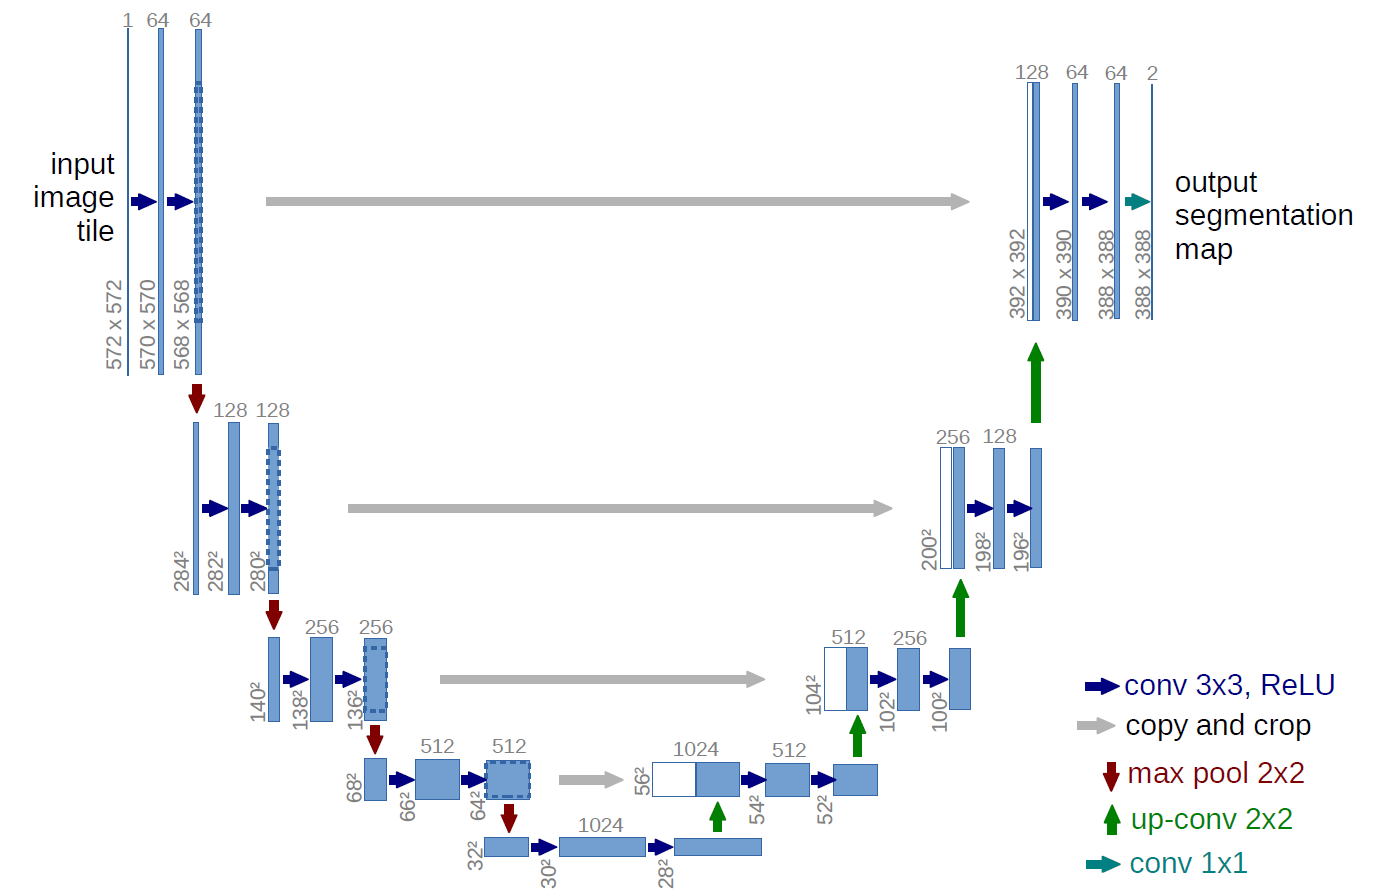
\includegraphics[width=\linewidth]{figures/chap223_unet.png}
	\caption[U-Net]{
		U-Net architecture. The left part of the shown network architecture represents the encoder network, while the right part represents the decoder network. 
		In between, the skip connections establish additional lateral links (visualized in gray) between the encoder and decoder network. 
		The skip connections exist on several levels to persistently combine classification and localization information. 
		Copyright \copyright 2015 Springer Nature. Reprinted by permission from \cite{RF15-U-Net}.}
	\label{fig:ch2:sec2:unet}
\end{figure}

In the following the effect of skip connections is exemplary demonstrated by the \gls{fcn} introduced in \cite{LSD15-FCN}.
The \gls{fcn} is based on the encoder-decoder-architecture with a relatively small decoder.
To compensate the absence of a deep decoder and refine the network, Long applies skip connections, that combine lower layers with the final prediction layer.
In order to compare the effect of skip connections, three models are created: one without skip-connection (\gls{fcn}-32s) and two with skip connection (\gls{fcn}-16s and \gls{fcn}-8s).
The number indicates the upsampling factor required from this point to the final predictions.
The \gls{fcn}-16s and \gls{fcn}-8s require less upsampling, due to their fusion with a lower layer.
\begin{figure}
	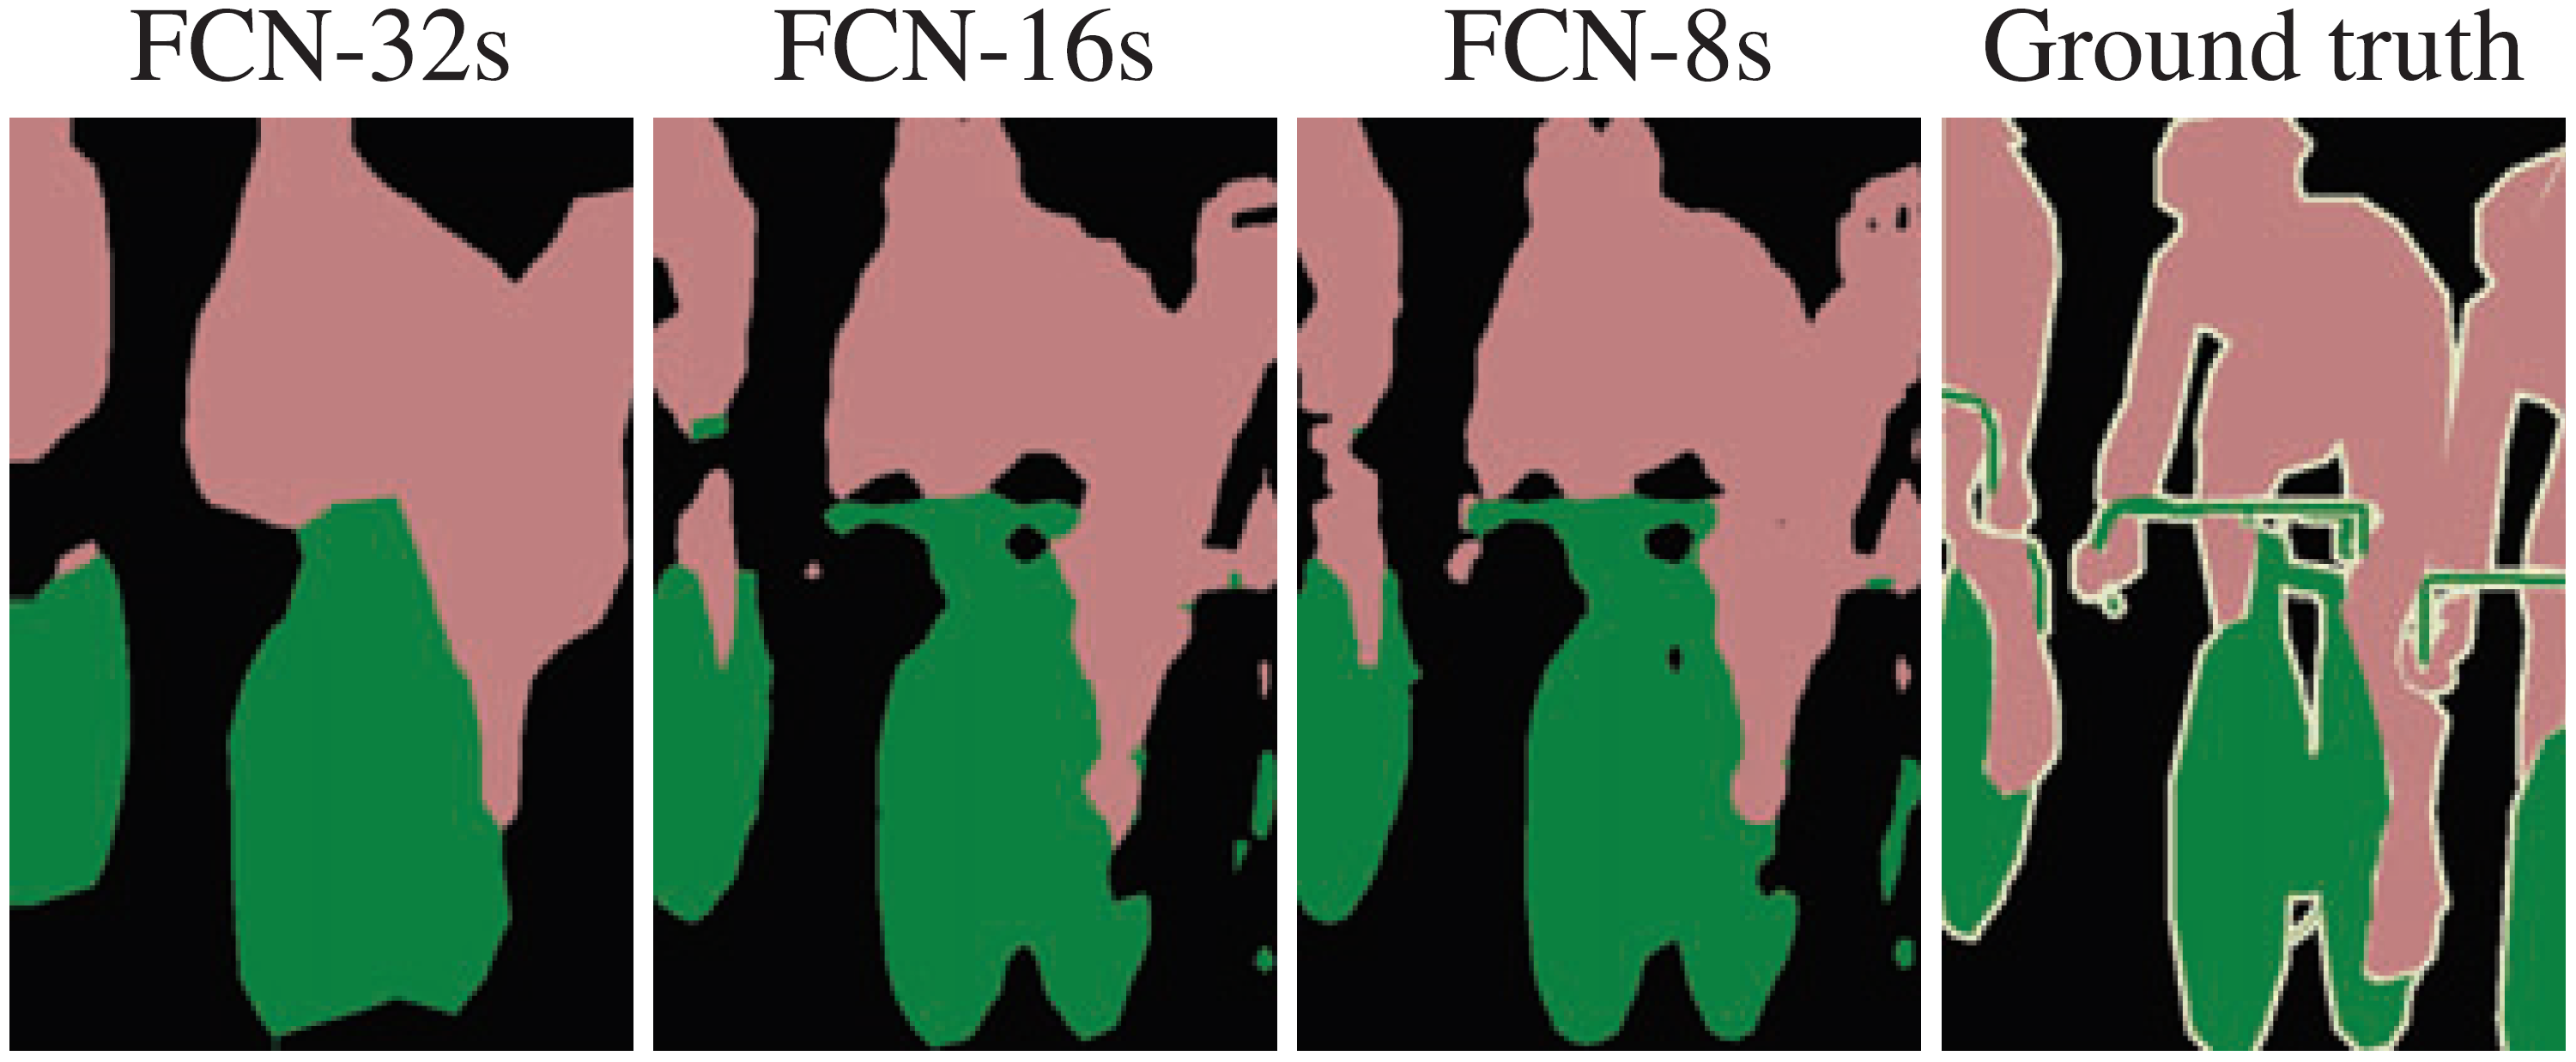
\includegraphics[width=\linewidth]{figures/chap223_fcn_results.png}	
	\caption[FCN Predictions]{
		Results of several variants of the \gls{fcn}. 
		It can be observed that the \gls{fcn}-32s creates a relatively coarse prediction compared to the networks with skip connections.
		In contrast the \gls{fcn}-8s achieves the best result with significantly improved level of detail and sharper borders.
		Copyright \copyright 2015 IEEE. Reprinted by permission from \cite{LSD15-FCN}.}
	\label{fig:ch2:sec2:fcn_res}
\end{figure}
The results shown in Figure \ref{fig:ch2:sec2:fcn_res} highlight the effect of skip connections in order to solve the question of localization.

\subsubsection{Pyramid Scene Parsing Network}

Another architectural component is introduced with the \gls{psp} network in \cite{Zhao17-PSP}.
% Problem / disadvantage of missing gobal context / subregions information
In this work it is stated, that the inclusion of more context information improves segmentation networks.
The quantity of the used context information is approximately indicated by the receptive field, which is size of the processed input region.
To enrich the context information it is proposed to combine the context information of several subregions.

This idea is based on \cite{He15-SPP}, where feature maps were processed by spatial pyramid pooling and thereby removed the limitations of fixed size.

% Idea: fused information from different subregions
To improve the context information, different subregions can be fused, similar as in 
% similar to \cite{He15-SPP} -> removes the fixed size contraint from CNNs

In \cite{Zhao17-PSP} this approach is further developed, by a hierarchical structure using multiple processing streams, also referred to as pyramid levels.
Each pyramid level processes the same feature map in various sizes.
Thereby, pooling layers with different filter sizes are applied to create feature maps of different sizes.
These feature maps are futher processed by convolutional layers and afterwards upsampled to a mutual size.
Last, the feature maps from the \gls{psp} module are concatenated with another and the features maps from the earlier processing step, as illustrated in Figure \ref{fig:ch2:sec2:psp}.
This \gls{psp} module enables the model to use more contextual information and therefore, improve the segmentation result.
\begin{figure}
	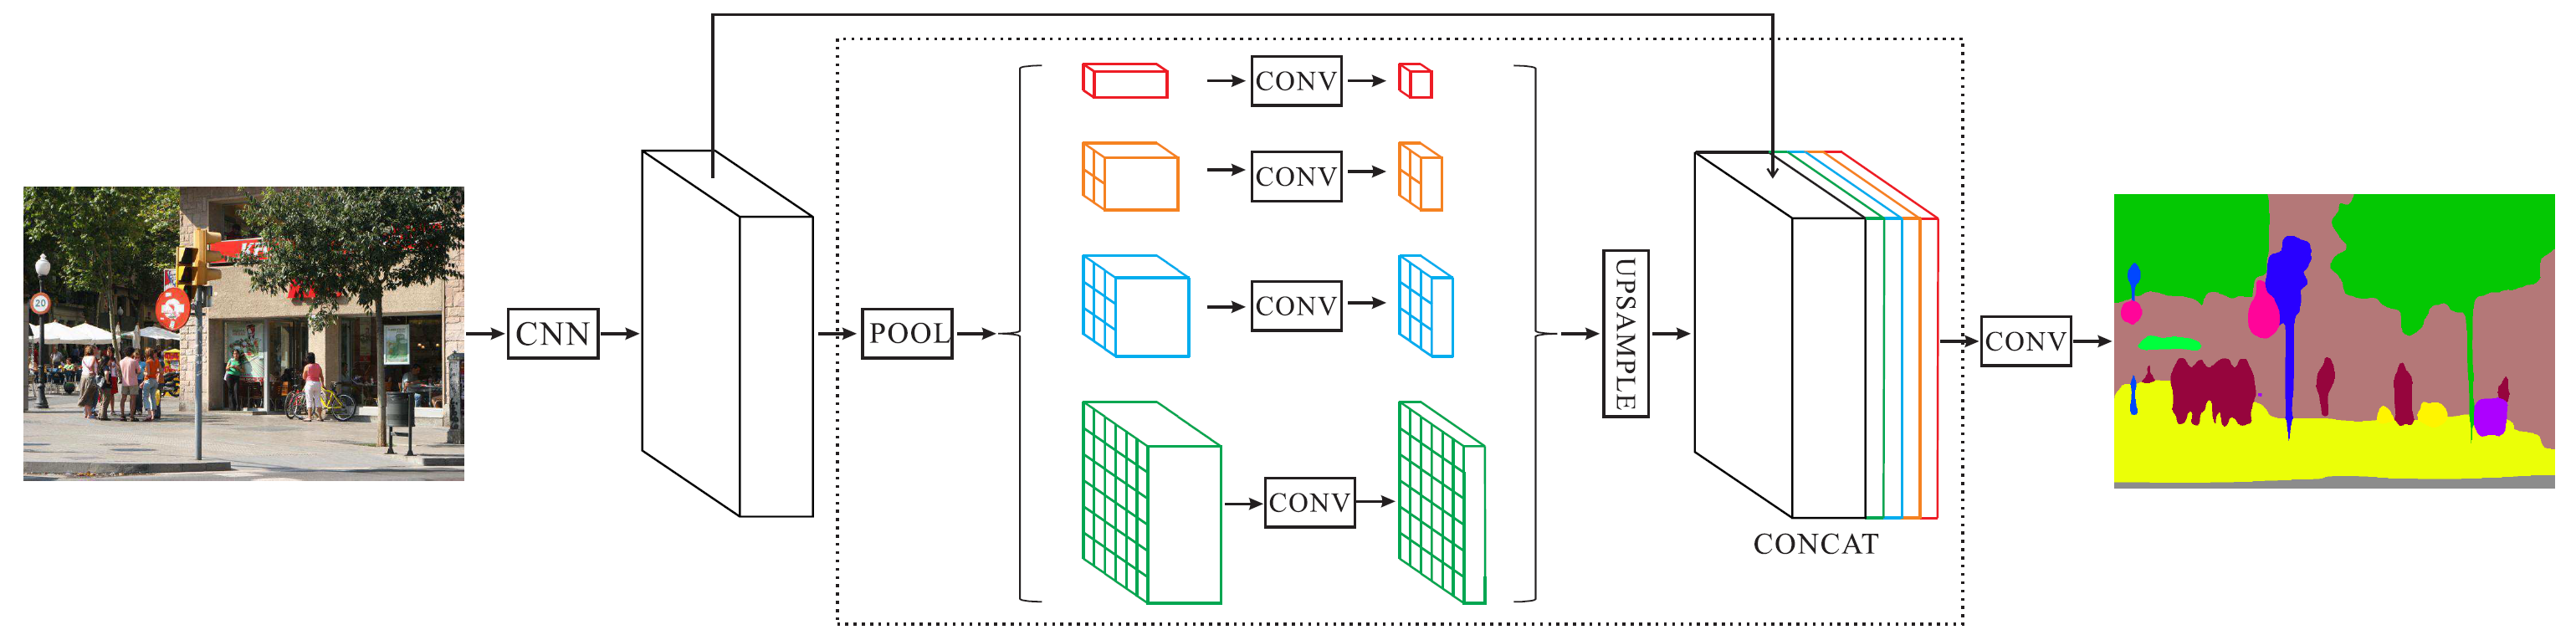
\includegraphics[width=\linewidth]{figures/chap223_psp.png}
	\caption[Pyramid Scene Parsing Network]{
		\gls{psp} Network with the pyramid pooling module in the middle.
		At (a) is the input image, which is fed into a \gls{cnn} for which a ResNet is used. 
		The feature maps (b) are the output of this \gls{cnn} and further processed in the pyramid pooling module (c).
		First, pooling with various sizes is applied, to create four feature maps of various sized, illustrated in different colors.
		These four feature maps are processed in the four pyramid level by convolutional layers.
		The respective sizes of the pyramid levels are $1 \times 1$, $2 \times 2$, $3 \times 3$ and  $6 \times 6$.
		The number of pyramid levels and their size can be modified.
		The results are upsampled to a mutual size and concatenated with another and the feature maps from (b).
		After the concatenation a final convolution is applied, which results in the final prediction (d) in the form of a segmentation map.
		Copyright \copyright 2015 IEEE. Reprinted by permission from \cite{Zhao17-PSP}.}
	\label{fig:ch2:sec2:psp}
\end{figure}



\subsubsection{DeepLab}
DeepLab is a \gls{dl} model for semantic segmentation developed by researchers from Google and first published in \cite{Chen16-DeepLab}.
It stands out due to the three techniques atrous convolution, \gls{aspp} \cite{He15-SPP} and, \gls{crf} \cite{KK12-CRF}, which are described in detail in \cite{Chen16-DeepLab}.
These techniques focus on the image's reconstruction in the upsampling process and therefore, improve the performance of the network.
A further development of these techniques is the DeepLabv3+ \cite{Chen18-DeepLab3+}, which set new performance records in 2018.

% \textbf{Atrous convolution} or dilated convolution modifies the kernel used for the convolution operation.	  The size of the kernel is extended and the upcoming gaps between the parameters are filled up with zeros.	The benefit is the coverage of a greater receptive field, without increasing the number of convolution parameters and so the computational load.
% \textbf{\gls{aspp}} is based on the concept of \gls{spp} introduced in \cite{He15-SPP}. 	\gls{spp} aims to combine images of different resolutions in order to obtain multi-scale information without increasing the computation time.	\gls{aspp} applies atrous convolution to the concept of \gls{spp}.	An input is fed into atrous convolution layers with different kernel sizes and the result is their combined output.
	
% \textbf{\gls{crf}} is statistical modeling method applied in \gls{ml}. \glspl{crf} aim to achieve sharper boundaries by considering the surrounding pixels before performing classification.		The functionality can be reviewed in detail in \cite{Chen16-DeepLab} and \cite{KK12-CRF}.	In contrast to most other segmentation models DeepLab does not use skip connections, but instead relies on \gls{crf} in order to recover fine details and the boundaries of objects to answer the question of localization.


\subsection{Data}\label{ord:ch2:sec2:subsec_data}
As image segmentation is a problem of supervised learning, a dataset with \gls{gt} is required.
For a dataset to be suitable in the field of \gls{dl} among others the following criteria should be met: size, quality and representation capability.
\begin{itemize}
	% Quantity data - size matters.
	\item The size of images within a dataset used for training a \gls{dl} model is crucial for its success.
	In general, small datasets, may not cover all vital characteristics to completely map a given objective.
	It has been shown in \cite{Banko01-ScalingData}, that the performance of networks can improve significantly using larger datasets for training.
	Also, in \cite{Halevy09-UnreasonableEffectivenessOfData} the effect of larger datasets is examined. 
	It is claimed that, using a larger dataset for training can improve the network's performance more than modifying the architecture of the network \cite{Ger17-HandsOn}.
	This highlights the importance of datasets with sufficient quantity to increase the performance of networks.
	% Quality data.
	\item The quality of the training data has a high impact on the model performance as well.
	Data, that is inconsistent, incomplete, erroneous, or too noisy, can lead to a significant decrease in performance \cite{Gudivada2017-DataQuality}.
	Training with poor quality data makes it more difficult for a model to detect and understand the elemental features and patterns, that are required by a model to perform well \cite{Ger17-HandsOn}.
	% TODO affect of poor quality data for object detection or segmentation segmentation. "With respect to the task of segmentation segmentation correctness is very significant, for the accuracy of the edges is crucial if a pixel is labelled with the correct class or not."	
	% Representative data.
	\item The capability of dataset to represent a given problem is another elemental characteristic.
	To enable a model to generalize and perform well, it is essential for the training data to be representative for the problem \cite{Ger17-HandsOn}.
	Goodfellow \etal also states, that the performance of a \gls{dl} model is strongly connected to the representation of the data \cite{Goodfellow-et-al-2016}.
	The best approach to do so, is to include samples of this specific problem or of samples from the same domain.	
	
	If the given problem is not represented within the samples of the used datasets, this may cause a decrease in performance.
	This may happen if a specific problem should be solved by a model, that is trained on general 'all-use-datasets', like PASCAL \gls{voc} \cite{Eve20-PascalVOC}, COCO \cite{Lin14-Coco} or ImageNet \cite{Deng09-ImageNet}.
	Therefore, it is important to pay attention to representation capability of the used dataset.
	% TODO \cite{Xu16-InteractiveObjectSelection}  The performance is evaluated on MS COCO with seen and unseen categories. Two points can be seen here: 	1. The significant drop in IU (Intersection over Union) from seen to unseen categories.  2. This network using user interaction suffers a way smaller drop in IU.
	%	For example, the aim of a DL model may be to detect a certain manufacturing part from an industrial scope.
	%	But without a dataset that represents this problem well enough, by containing samples from industrial scopes, the performance of the DL model may be significantly worse.
	%	This may results in a decrease of performance, because the capabilities of \gls{dl} models are strongly connected with the representation of the data \cite{Goodfellow-et-al-2016}.
\end{itemize} 
% Very hard and expensive to obtain data for segmentation and special domains.
It is a challenge to obtain a dataset, that meets these criteria.
The acquisition of new image datasets is very expensive in time and cost.
Datasets for semantic segmentation are even more expensive due to the high effort required to label images on pixel-level.
Especially, uncommon or confidential domains (\eg medical or industrial domains) are rarely covered in public datasets.
For example, the manufacturing process in a closed industrial environment may contain unique objects or uncommon surroundings, that are hardly ever represented in large-scale, open source datasets.

% New ways to obtain GT -> Labeltool, Interactive methods, AI-Simulation 
New approaches have been created, to facilitate the process of creating new dataset and label images with pixel-level accuracy.
An efficient and common way is a program, that simplifies labeling process by providing a user interface and multiple methods to create and save label.

Specific \textit{label} or \textit{annotation tools} provide a user interface and easy-to-use methods to create and edit labels. 
Due to the hight demand for labeled training data there are various labeltools available.\footnote{E. Cerna, \textit{Image Annotation Tools: Which One to Pick in 2020?} \url{https://bohemian.ai/blog/image-annotation-tools-which-one-pick-2020/}}
To simplify the manual process of labeling for a human user interactive methods facilitate the label process (see Chapter \ref{ord:ch2:sec3}).
Another approach is to create synthetic datasets like the SYNTHIA dataset \cite{Zol19-Temporal} and use them for training of semantic segmentation networks \cite{Chen18-SyntheticData}.


\subsection{State-of-the-art}\label{ord:ch2:sec2:subsec_compare}

An overview about the performance of previously introduced and current state-of-the-art networks is given in Table \ref{tab:ch2:stae-of-the-art}.
As benchmark dataset the PASCAL \gls{voc} test set \cite{Eve20-PascalVOC} and as metric the \gls{miou} were selected, due to their widespread usage.
Notable is the rapid increase of performance over the last years, which emphasizes the relevance and research interest on this field of study.
The model delivering the best performance is currently the EfficientNet introduced in \cite{Zoph20-EfficientNet}, which is superior due to the application of so-called \textit{self-training}.
\begin{table}[h!]
	\centering
	\begin{tabular}{l|r}
		\textbf{Model} 								& \textbf{mIoU}\\
		\hline
		\gls{fcn}-8s \cite{LSD15-FCN} 				& 62.2\\
		DeconvNet \cite{NHH15-DeConvNet}			& 72.5\\
		DeepLab-CRF \Cite{Chen16-DeepLab} 			& 79.7\\
		\gls{psp}Net \cite{Zhao17-PSP}				& 85.4\\
		DeepLabv3+ \cite{Chen18-DeepLab3+} 			& 87.8\\
		EfficientNet \cite{Zoph20-EfficientNet} 	& 90.5\\
	\end{tabular}
	\caption[Comparison of image segmentation models]{
		Comparison of image segmentation models on the PASCAL \gls{voc} 2012 test set.
		It has to be noted, that the \gls{miou} is calculated with application of \gls{vp} from PASCAL \gls{voc}.
		An more detailed overview with all officially submitted models can be reviewed PASCAL \gls{voc} 2012 leaderboard.\footnotemark 
	}
	\label{tab:ch2:stae-of-the-art}
\end{table}
\footnotetext{Segmentation Results: Leaderboard PASCAL \gls{voc} 2012: \url{http://host.robots.ox.ac.uk:8080/leaderboard/displaylb_main.php?challengeid=11&compid=6}}
%TODO ensure the footnote is on the same page as the table